\documentclass[paper=a4, fontsize=11pt, onecolumn, tikz, dvipsnames, svgnames, x11names]{article}
\usepackage[utf8]{inputenc}
\usepackage[T1]{fontenc}
\usepackage[english]{babel}
\usepackage{multicol}
\usepackage{fullpage}
% ------------------------- Color table ----------------------------------------
\usepackage{multirow}
\usepackage[table]{xcolor}
\definecolor{maroon}{cmyk}{0,0.87,0.68,0.32}
\usepackage{booktabs} % to make prettier tables (toprule, midrule, bottomrule)
% ------------------------------------------------------------------------------

\usepackage{amscd}
\usepackage{amsthm}
\usepackage{physics}
\usepackage{textcomp,gensymb} %pour le °C, et textcomp pour éviter les warning
\usepackage{graphicx} %pour les images
\usepackage{caption}
\usepackage{subcaption}
\usepackage[colorlinks=true,
	breaklinks=true,
	citecolor=blue,
	linkcolor=blue,
	urlcolor=blue]{hyperref} % pour insérer des liens
\usepackage{epstopdf} %converting to PDF
\usepackage[export]{adjustbox} %for large figures

\usepackage{array}
\usepackage{dsfont}% indicatrice : \mathds{1}


% -------------------------- Mathematics ---------------------------------------
\graphicspath{{images/}{../images/}} % For the images path
% ------------------------------------------------------------------------------

% -------------------------- Mathematics ---------------------------------------
\usepackage{mathrsfs, amsmath, amsfonts, amssymb}
\usepackage{bm}
\usepackage{mathtools}
\usepackage[Symbol]{upgreek} % For pi \uppi different from /pi
\newcommand{\R}{\mathbb{R}} % For Real space
\usepackage{tikz}
\usetikzlibrary{bayesnet} %library to draw graphical models1
% ------------------------------------------------------------------------------


% -------------------------- Code format ---------------------------------------
\usepackage[numbered,framed]{matlab-prettifier}
\lstset{
	style              = Matlab-editor,
	basicstyle         = \mlttfamily,
	escapechar         = '',
	mlshowsectionrules = true,
}
% ------------------------------------------------------------------------------

% ------------------------- Blbiographie --------------------------------------
% \usepackage[backend=biber, style=ieee]{biblatex}
% \addbibresource{biblio.bib}
% \bibliography{../material/biblio.bib}
% \usepackage{csquotes}
% ------------------------------------------------------------------------------


\setcounter{tocdepth}{4} %Count paragraph
\setcounter{secnumdepth}{4} %Count paragraph
\usepackage{float}

\usepackage{graphicx} % for graphicspath
% \graphicspath{{../images/}}

\usepackage{array,tabularx}
\newcolumntype{L}[1]{>{\raggedright\let\newline\\\arraybackslash\hspace{0pt}}m{#1}}
\newcolumntype{C}[1]{>{\centering\let\newline\\\arraybackslash\hspace{0pt}}m{#1}}
\newcolumntype{R}[1]{>{\raggedleft\let\newline\\\arraybackslash\hspace{0pt}}m{#1}}


% \usepackage{algpseudocode}
% \usepackage{algorithm}
\usepackage{hyperref}
\usepackage[edges]{forest}

% ------------------------------ Jules packages --------------------------------
\usepackage[ruled,vlined]{algorithm2e}
\usepackage[colorinlistoftodos]{todonotes}
\usepackage{alltt}

% Independent sign
\newcommand{\indep}{\ensuremath{\,\bot\!\!\!\bot\,}} %% The symbol for independent

% Alpha / Numbers for sections
\renewcommand{\thesubsubsection}{\arabic{section}.\arabic{subsection}.\alph{subsubsection})}

\newcommand{\argmin}[1]{\underset{#1}{\operatorname{argmin}}\;}

% % Norm
% \newcommand{\norm}[1]{\left\lVert#1\right\rVert}


% ------------------------ General informations --------------------------------
\title{\normalfont \normalsize \huge Pointing error correction}
\author{Jules Kozolinsky, Vincent Matthys}
\graphicspath{{images/}{../images/}} % For the images path
% ------------------------------------------------------------------------------


\date{}

\begin{document}
%\maketitle

 \begin{tabularx}{0.9\textwidth}{@{} l X r @{} }
 	{\textsc{Master MVA}}  &  & \textsc{} \\
 	\textsc{Remote sensing} &  & {ENS Paris Saclay}       \\
 \end{tabularx}
 \vspace{1.5cm}
 \begin{center}

 	\rule[11pt]{5cm}{0.5pt}

 	\textbf{\LARGE \textsc{Pointing error correction}}
 	\vspace{0.5cm}

 	Jules Kozolinsky,
 	Vincent Matthys

 	\href{mailto:jules.kozolinsky@ens-cachan.fr}{jules.kozolinsky@ens-cachan.fr} \\
 	\href{mailto:vincent.matthys@ens-paris-saclay.fr}{vincent.matthys@ens-paris-saclay.fr}

 	\rule{5cm}{0.5pt}

 	\vspace{1.5cm}
 \end{center}

 \tableofcontents

\section{Attitude of a Satellite}

\begin{figure}[h]
    \centering
    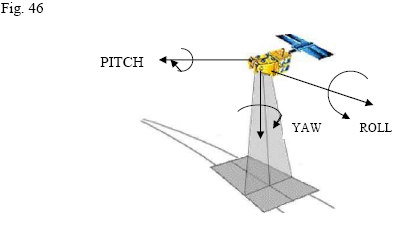
\includegraphics[width=0.5\textwidth]{figures/angles.jpg}
   \caption{ Roll, pitch and yaw angles.}
   \label{angles}
\end{figure}

\section{Satellite attitude error effects on stereo images}
\label{sec:sensibility}
What is pointing error ?
Sensiblity of roll, pitch and yaw. Scheme (roll and pitch depend of the height of the satellite whereas yaw only the angle)


\section{Correction of Relative Pointing Error}
\cite{carlo_2014_pushbroom}\\

A simple way to correct the relative pointing error is to transform one of the two images, in such a way that the corresponding points fall on the respective epipolar curves: given two images $u$, $v$ and a set of correspondences $(\textbf{x}_i , \textbf{x}'_i)_{i=1...N}$ , we search for a transformation $f$ such that, for all $i$, the transformed point $f(\textbf{x}'_i)$ lies on the epipolar curve $\text{epi}^{\textbf{x}_i}_{u v}(R)$.
The desired transformation $f^{*}$ minimises the relative pointing error:
\begin{align}
\label{minif}
f^* = \argmin{f} \dfrac{1}{N} \sum\limits_{i=1}^{N} d(f(\textbf{x}'_i), \text{epi}^{\textbf{x}_i}_{u v}(R))
\end{align}

\paragraph{Affine fundamental matrix approximation\\}
From  \cite{carlo_2014_pushbroom}, we know that, for each correspondence $i$, the epipolar curve $\text{epi}^{\textbf{x}_i}_{u v}(R)$ is approximated up to $0.05$ pixels by the straight line $F\textbf{x}_i$, where $F$ is
the affine fundamental matrix between the two views for the considered tile. Since the fundamental matrix, due to the approximation, is \textit{affine}, all the lines $(F\textbf{x}_i)_{i=1...N}$ are parallel.

\subsection{Roll and Pitch Angles}
Because of sensitivity issues, we first can take only roll and pitch error into account. Therefore, according to section \ref{sec:sensibility}, we search for a transformation $f$ such that
\begin{align*}
f(\textbf{x}) = T\textbf{x}
\end{align*}
where $T$ is a translation:
\begin{align*}
T =
\begin{pmatrix}
1 & 0 & t_x \\
0 & 1 & t_y \\
0 & 0 & 1
\end{pmatrix}
\end{align*}
We can write the transformation $f$, for $ \textbf{x} = (  x \; y \; 1)^T $, as:
\begin{align*}
f(\textbf{x}) = T\textbf{x} =
\begin{pmatrix}
x + t_1 \\
y + t_2 \\
1
\end{pmatrix}
\end{align*}


Without any additional restriction, we may assume that these lines are horizontal (otherwise just do a change of coordinates). This change of coordinates is called \textit{rectification}. We find \\%TODO explain rectification

After rectification, for each point $i$, the horizontal line $F\textbf{x}_i$ can be written as
\begin{align*}
F\textbf{x}_i = \left[ 0 \; 1 \; c_i \right]
\end{align*}
With these notations, for each point correspondence $(\textbf{x}_i , \textbf{x}'_i)$, the pointing error $e$ is:
\begin{align*}
e(\textbf{x}_i, \textbf{x}'_i) = d(\textbf{x}'_i, epi^{\textbf{x}_i}_{u v}(R)) = d(\textbf{x}'_i, F\textbf{x}_i) = | y'_i + c_i|
\end{align*}

Here the error $e$ is invariant to any horizontal translation, thus the search for a translation minimizing the relative pointing error of formula (\ref{minif}) can be restricted to vertical translations only. With a vertical translation of parameter $t$, the global pointing error becomes
\begin{align*}
E = \dfrac{1}{N} \sum\limits_{i=1}^{N} d(T\textbf{x}'_i, F\textbf{x}_i) = \dfrac{1}{N} \sum\limits_{i=1}^{N} | y'_i + t+ c_i|
\end{align*}
The translation that minimizes this sum is given by the geometric median (Weiszfeld, 1937) of the vector $(-y'_i - c_i )_{i=1...N}$.  The pointing error can thus be minimized by applying a translation to one of the images. Note that the median is robust against outliers, thus this correction procedure works well even in the presence of false matches.


\subsection{Roll, Pitch and Yaw Angles}
If we assume that the scene is located at infinity with respect to the satellite, an error in the sensor attitude measurement can be modeled in image space as a translation composed with a rotation. Therefore we have
\begin{align*}
f(\textbf{x}) = TR\textbf{x}
\end{align*}
where $R$ is a rotation and $T$ a translation:\\
\begin{align*}
R =
\begin{pmatrix}
\cos(\theta) & -\sin(\theta) & 0 \\
\sin(\theta) & \cos(\theta) & 0 \\
0 & 0 & 1
\end{pmatrix}, \;
T =
\begin{pmatrix}
1 & 0 & t_x \\
0 & 1 & t_y \\
0 & 0 & 1
\end{pmatrix}
\end{align*}

\subsubsection{Approximation of the Rotation}

To correct the pointing error in the rectified setting we find $R^*$ and $T^*$ minimizing the pointing error defined as follow :
\begin{align}
    (R^*, T^*) = \argmin{R,T} \sum_{i=1}^N d(TR\bm{x_i'}, F\bm{x}_i)^2
\end{align}
As in~\cite{carlo_2014_automatic}

After rectification, the horizontal line $F\bm{x}_i$ can be written, in homogeneous coordinates, as
\begin{align*}
F\bm{x}_i =  \begin{bmatrix} 0 & 1 & y_i \end{bmatrix}
\end{align*}
With these notations, if the model now includes a rotation $R$, for each point correspondence $(\bm{x}_i , \bm{x}'_i)$, we have
\begin{align*}
e(\textbf{x}_i, \textbf{x}'_i) = d(TR\bm{x}'_i, \text{epi}^{\bm{x}_i}_{u v}(R)) = d(TR\bm{x}'_i, F\bm{x}_i) = |x_i' \sin \theta   + y_i' \cos \theta  + t - y_i |
\end{align*}
where $\theta$ is the angle of the rotation.

We can consider that $\theta$ is small enough compare to $2\pi$. In fact on satellites such as Sentinel or Pleiades (%TODO source)
the precision of the yaw angle is around $50~\mu \text{rad}$. Even if Planet's sensor would be $100$ less precise, we will still have an yaw angle less than $1$ degree.
With this approximation, we can write:
\begin{align*}
e(\textbf{x}_i, \textbf{x}'_i) = |x_i' \theta   + y_i' + t - y_i |
\end{align*}

Correcting the global pointing error is to minimize:
\begin{align*}
(\theta^*, t^*) = \argmin{\theta,t} \sum_{i=1}^N d(TR\bm{x_i'}, F\bm{x}_i)^2 = \sum_{i=1}^N (x_i' \theta   + y_i' + t - y_i)^2
\end{align*}
We can write this optimization problem as :
\begin{align*}
X^* = \argmin{X} \| AX + b \|^2
\end{align*}
where
\begin{align*}
A =
\begin{pmatrix}
x_1' & 1 \\
x_2' & 1 \\
\vdots & \vdots \\
x_n' & 1 \\
\end{pmatrix} \quad
X =
\begin{pmatrix}
\theta \\
t
\end{pmatrix} \quad
b =
\begin{pmatrix}
y_1' - y_1\\
y_2' - y_2\\
\vdots\\
y_1' - y_1\\
\end{pmatrix}
\end{align*}

The solution of this optimization problem is the solution of the normal equation
\begin{align*}
 A^TAX = -A^Tb
\end{align*}
Here,
\begin{align*}
A^TA =
\begin{pmatrix}
\sum\limits_{i=1}^N x_{i}'^2 & \sum\limits_{i=1}^Nx_{i}' \\
\sum\limits_{i=1}^N x_{i}' & N \\
\end{pmatrix}
\end{align*}
So $A^TA$ is inversible, and the optimal correction in the rectified images is:
\begin{align*}
\begin{pmatrix}
\theta^* \\
t^*
\end{pmatrix} = X^* = -(A^TA)^{-1}A^Tb
\end{align*}


\subsubsection{Solving Numerically an Optimization Problem}
To correct the pointing error in the rectified setting we find $R^*$ and $T^*$ minimizing the pointing error defined as follow :
\begin{align}
    (R^*, T^*) = \argmin{R,T} \sum_{i=1}^N d(RT\bm{x_i'}, F\bm{x}_i)
\end{align}

Since we are not able to solve this optimization problem analytically, we solve it numerically thanks to the L-BFGS algorithm. As input are the correspondences on the images and the affine approximation matrix and the optimization algorithm outputs the optimal angle $\theta \in [0, 2\pi]$ corresponding to the error on the yaw and a translation $t \in \mathbb{R}$ corresponding to a translation in the normal direction w.r.t. the epipolar lines.

\paragraph{Limited-memory BFGS\\}
Limited-memory BFGS is an optimization algorithm in the family of quasi-Newton methods that approximates the BFGS algorithm using a limited amount of computer memory. In our case we do not need to compute the gradient analytically since the algorithm approximates it using finite difference. We use this algorithm as a black box to solve the minimization problem.

\section{Data overview}

\subsection{Test data}

S2P pipeline comes with a pair and a triplet of test data captured by Pleiades. The input pair and their geolocalisation is shown below in figure~\ref{fig_geoloc_testdata}. After the pair, the triplet is also represented in figure~\ref{fig_geoloc_testdata_triplet}. The expected output result is also shown in figure~\ref{fig_expected_output_pair}, and is offline visuable using the PotreeConverter module available on github~\cite{PotreeConverter}.

\begin{figure}[H]
    \centering
    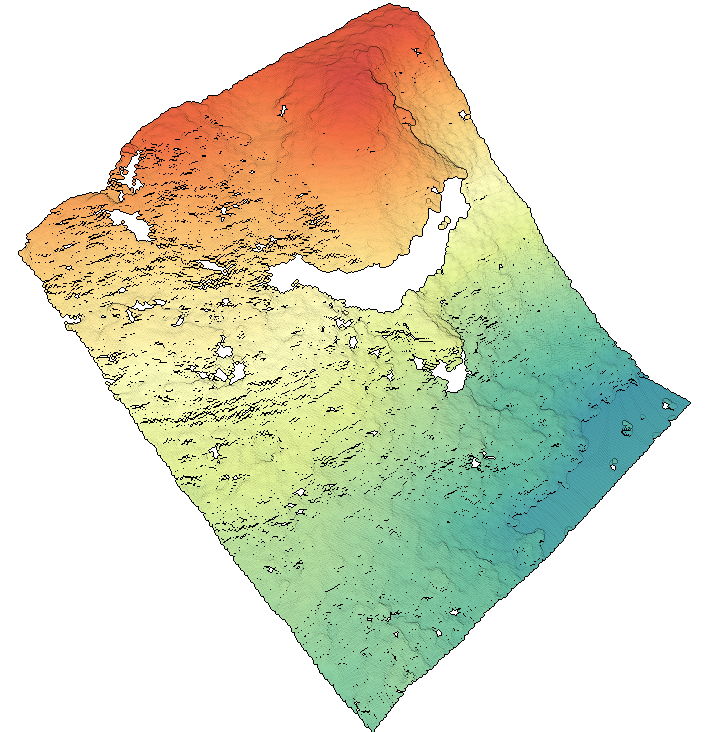
\includegraphics[height = 0.4\textheight]{elevation_intro.png}
    \caption{Expected output of S2P on test data input pair}
    \label{fig_expected_output_pair}
\end{figure}


\begin{figure}[H]
    \centering
    \begin{subfigure}[t]{0.8\textwidth}
        \centering
        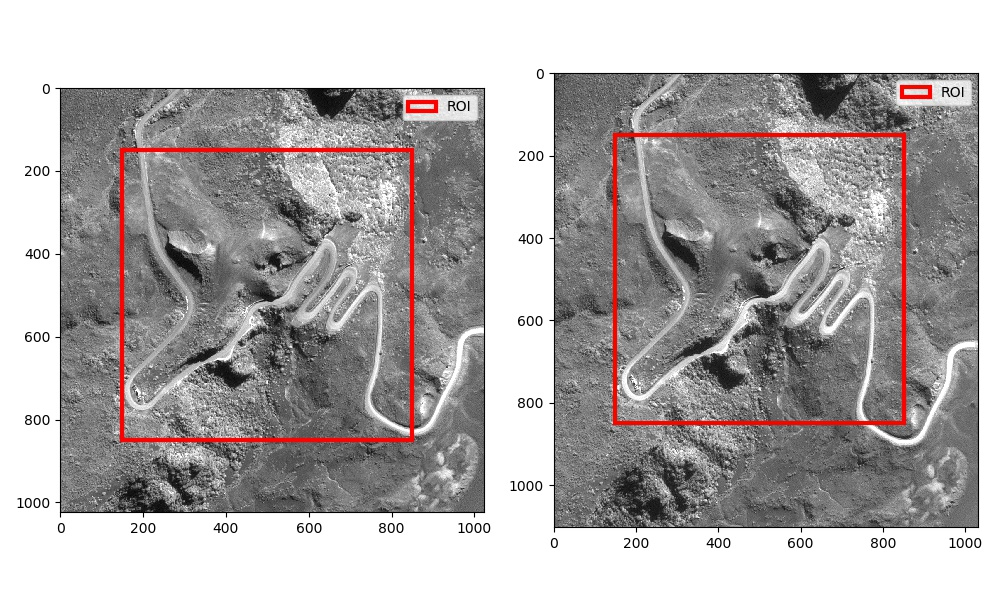
\includegraphics[width = 0.95\textwidth]{ROI_testdata_pair.jpeg}
        \caption{Region of intereset (ROI, in red) in test data input pair}
    \end{subfigure}%
    ~
    \vfill
    ~
    \begin{subfigure}[t]{0.8\textwidth}
        \centering
        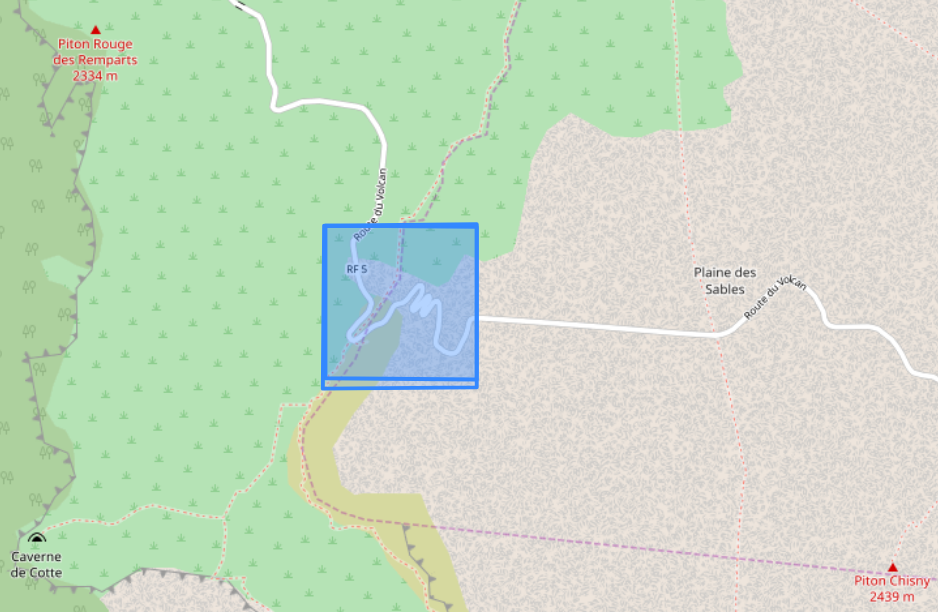
\includegraphics[width = 0.95\textwidth]{geoloc_testdata.png}
        \caption{Geolocalisation of the test data input pair, in La Réunion. Reprojected using an elevation of $h=2350~m$. Center of ROI $(lat, lon) ~\approx (-21.23066754, 55.65022517)$}
    \end{subfigure}%
    \caption{Overview of the test data input pair}
    \label{fig_geoloc_testdata}
\end{figure}

\begin{figure}[H]
    \centering
    \begin{subfigure}[t]{0.8\textwidth}
        \centering
        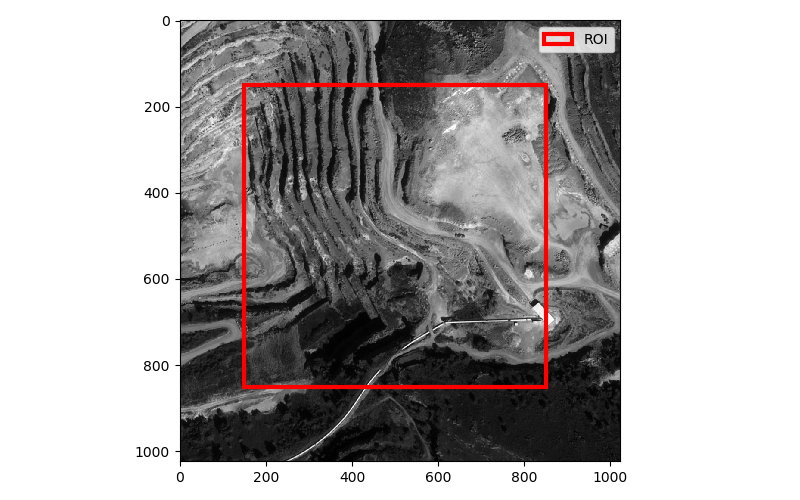
\includegraphics[width = 0.95\textwidth]{ROI_testdata_triplets.png}
        \caption{Region of intereset (ROI, in red) in test data input triplet. Only one (img\_01.tif) of the 3 images is represented.}
    \end{subfigure}%
    ~
    \vfill
    ~
    \begin{subfigure}[t]{0.8\textwidth}
        \centering
        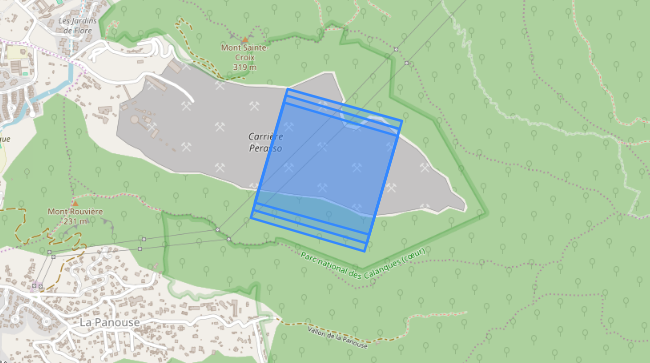
\includegraphics[width = 0.95\textwidth]{geoloc_testdata_triplets.png}
        \caption{Geolocalisation of the test data input triplet, east of Marseille. Reprojected using an elevation of $h=300~m$. Center of ROI $(lat, lon) ~\approx (43.26182762, 5.443071)$}
    \end{subfigure}%
    \caption{Overview of the test data input triplet}
    \label{fig_geoloc_testdata_triplet}
\end{figure}

\subsection{Planet Data}


\subsubsection{Structure}

The structure of the provided Skysat-2 data are represented in figure~\ref{fig_forest_skysat_2}.

\begin{figure}
    \begin{forest}
      my label/.style={
        label={[font=\sffamily]right:{#1}},
      },
      for tree={
        folder,
        font=\sffamily,
        text=white,
        minimum height=0.75cm,
        if level=0{fill=ForestGreen}{fill/.wrap pgfmath arg={SlateBlue#1}{int(4-(mod((level()-1),4)))}},
        rounded corners=4pt,
        grow'=0,
        edge={ForestGreen,rounded corners,line width=1pt},
        fit=band,
      },
      [data
        [s03\_20161003T161107Z
          [panchromatic
            [s03\_20161003T161107Z\_pan\_d1\_0001\_rpc.txt]
            [s03\_20161003T161107Z\_pan\_d1\_0001.tif]
          ]
          [pansharp
            [s03\_20161003T161107Z\_pansharp\_bgrn\_d1\_0001\_rpc.txt]
            [s03\_20161003T161107Z\_pansharp\_bgrn\_d1\_0001.tif]
          ]
        ]
        [s03\_20161003T161148Z
          [panchromatic
            [s03\_20161003T161148Z\_pan\_d1\_0001\_rpc.txt]
            [s03\_20161003T161148Z\_pan\_d1\_0001.tif]
          ]
          [pansharp
            [s03\_20161003T161148Z\_pansharp\_bgrn\_d1\_0001\_rpc.txt]
            [s03\_20161003T161148Z\_pansharp\_bgrn\_d1\_0001.tif]
          ]
        ]
        [s03\_20161003T161231Z
          [panchromatic
            [s03\_20161003T161231Z\_pan\_d1\_000\_rpc.txt]
            [s03\_20161003T161231Z\_pan\_d1\_0001.tif]
          ]
          [pansharp
            [s03\_20161003T161231Z\_pansharp\_bgrn\_d1\_0001\_rpc.txt]
            [s03\_20161003T161231Z\_pansharp\_bgrn\_d1\_0001.tif]
          ]
        ]
      ]
    \end{forest}
    \caption{Structure of the provided Skysat-2 data}
    \label{fig_forest_skysat_2}
\end{figure}

\subsubsection{Geolocalisation}

\newpage
\begin{figure}
    \centering
    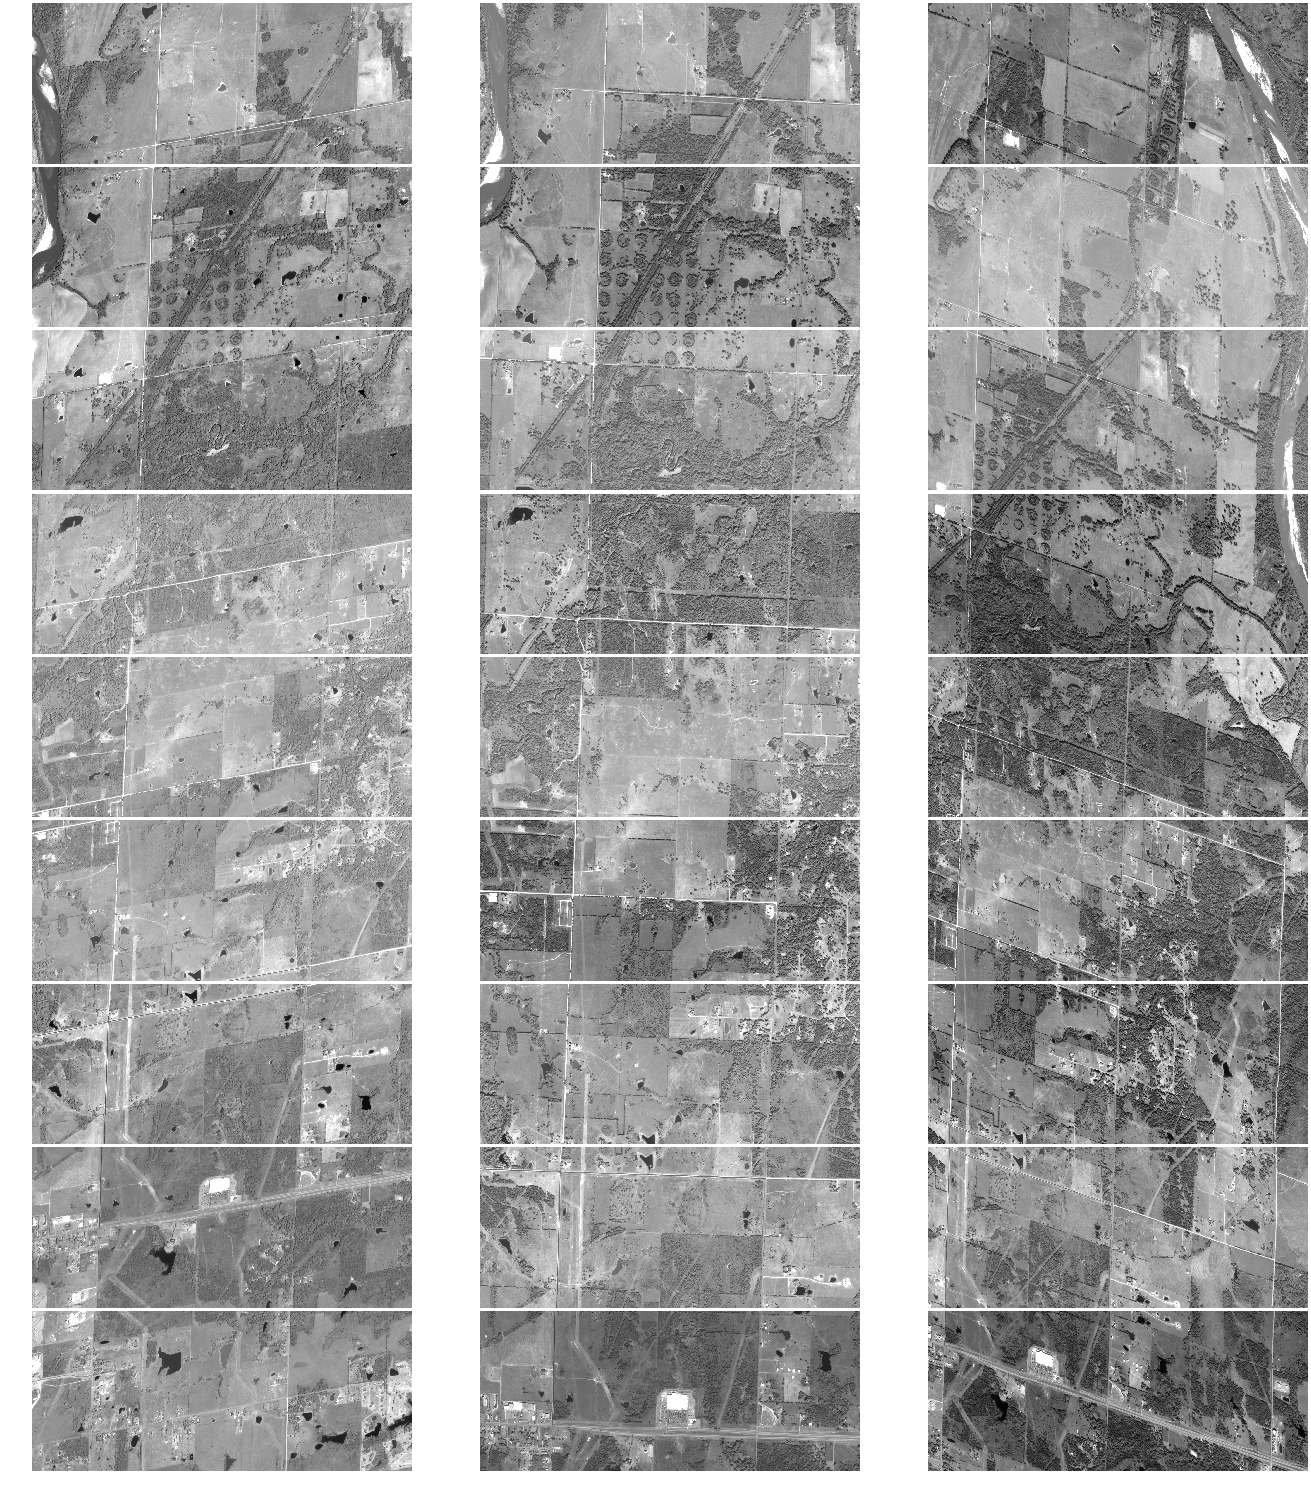
\includegraphics[width = 0.95\textwidth]{d1.png}
    \caption{Mosaic of d1. From left to right: 1Z, 8Z, 7Z}
    \label{fig_mosaic_d1}
\end{figure}

\newpage
\begin{figure}
    \centering
    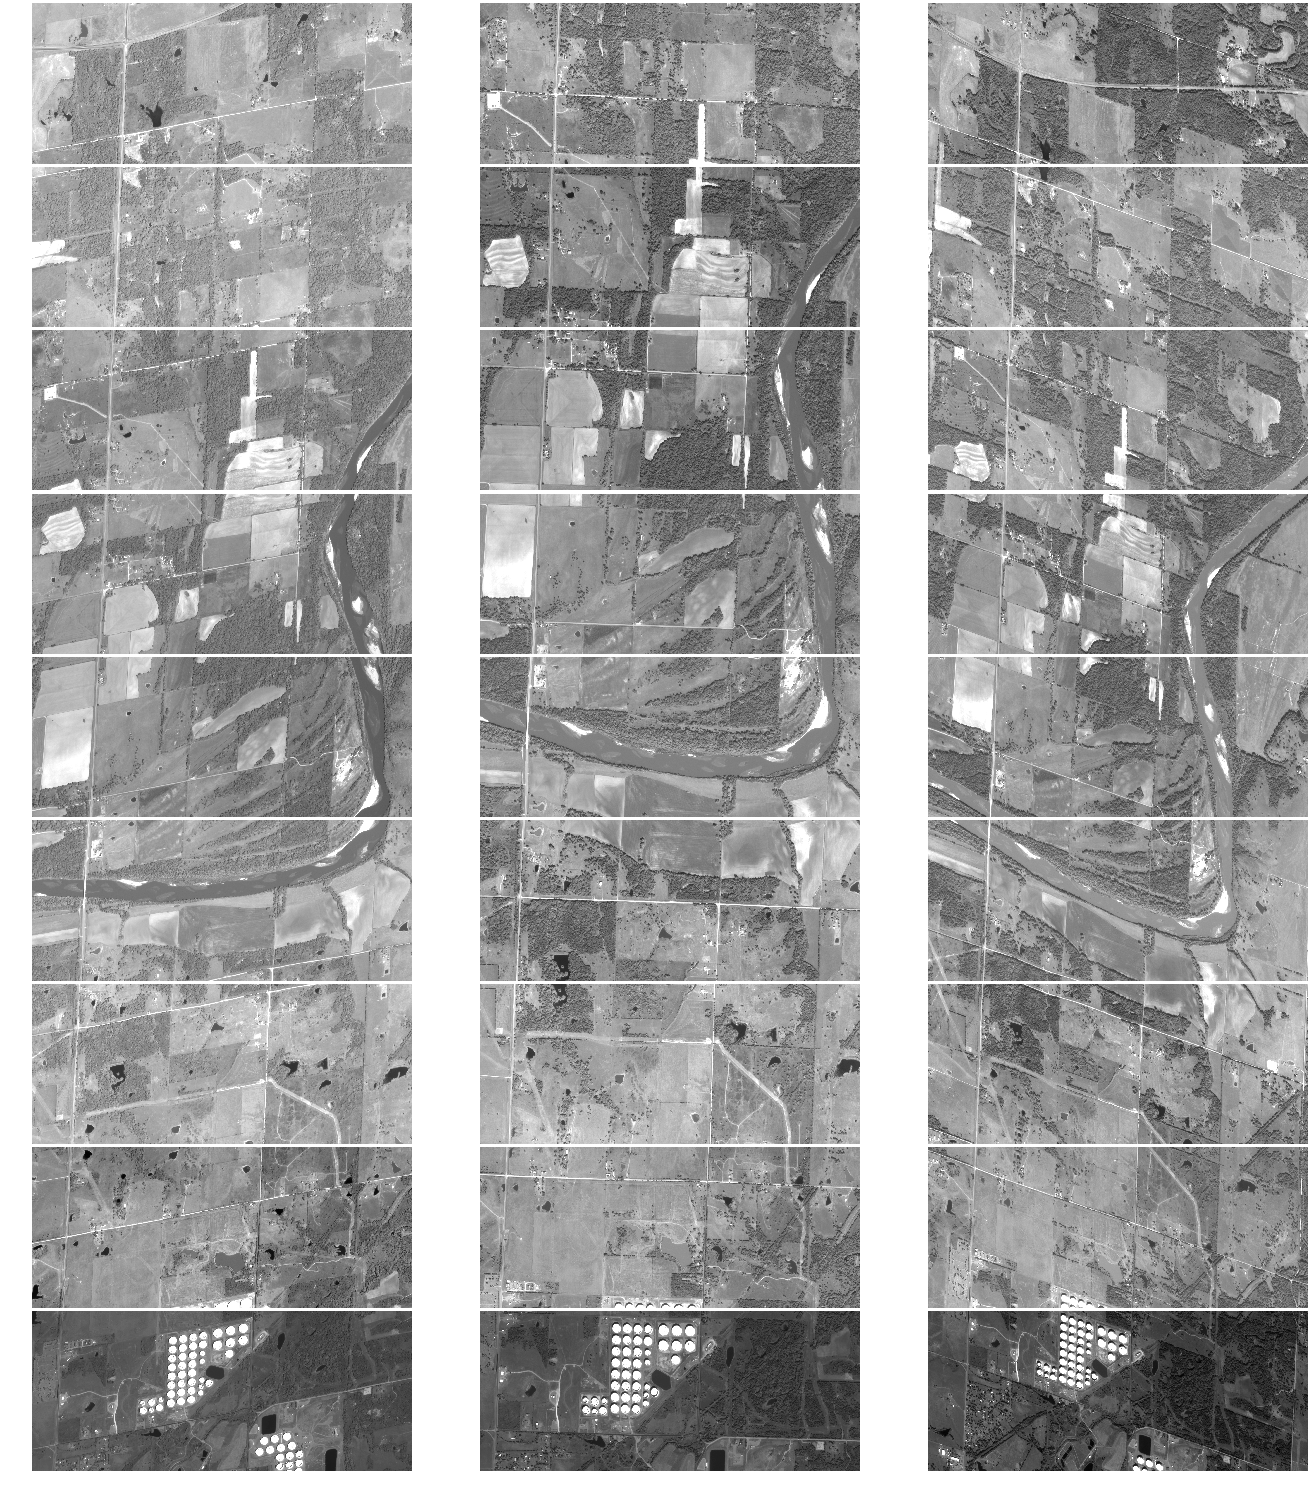
\includegraphics[width = 0.95\textwidth]{d2.png}
    \caption{Mosaic of d2. From left to right: 1Z, 8Z, 7Z}
    \label{fig_mosaic_d2}
\end{figure}

\newpage
\begin{figure}
    \centering
    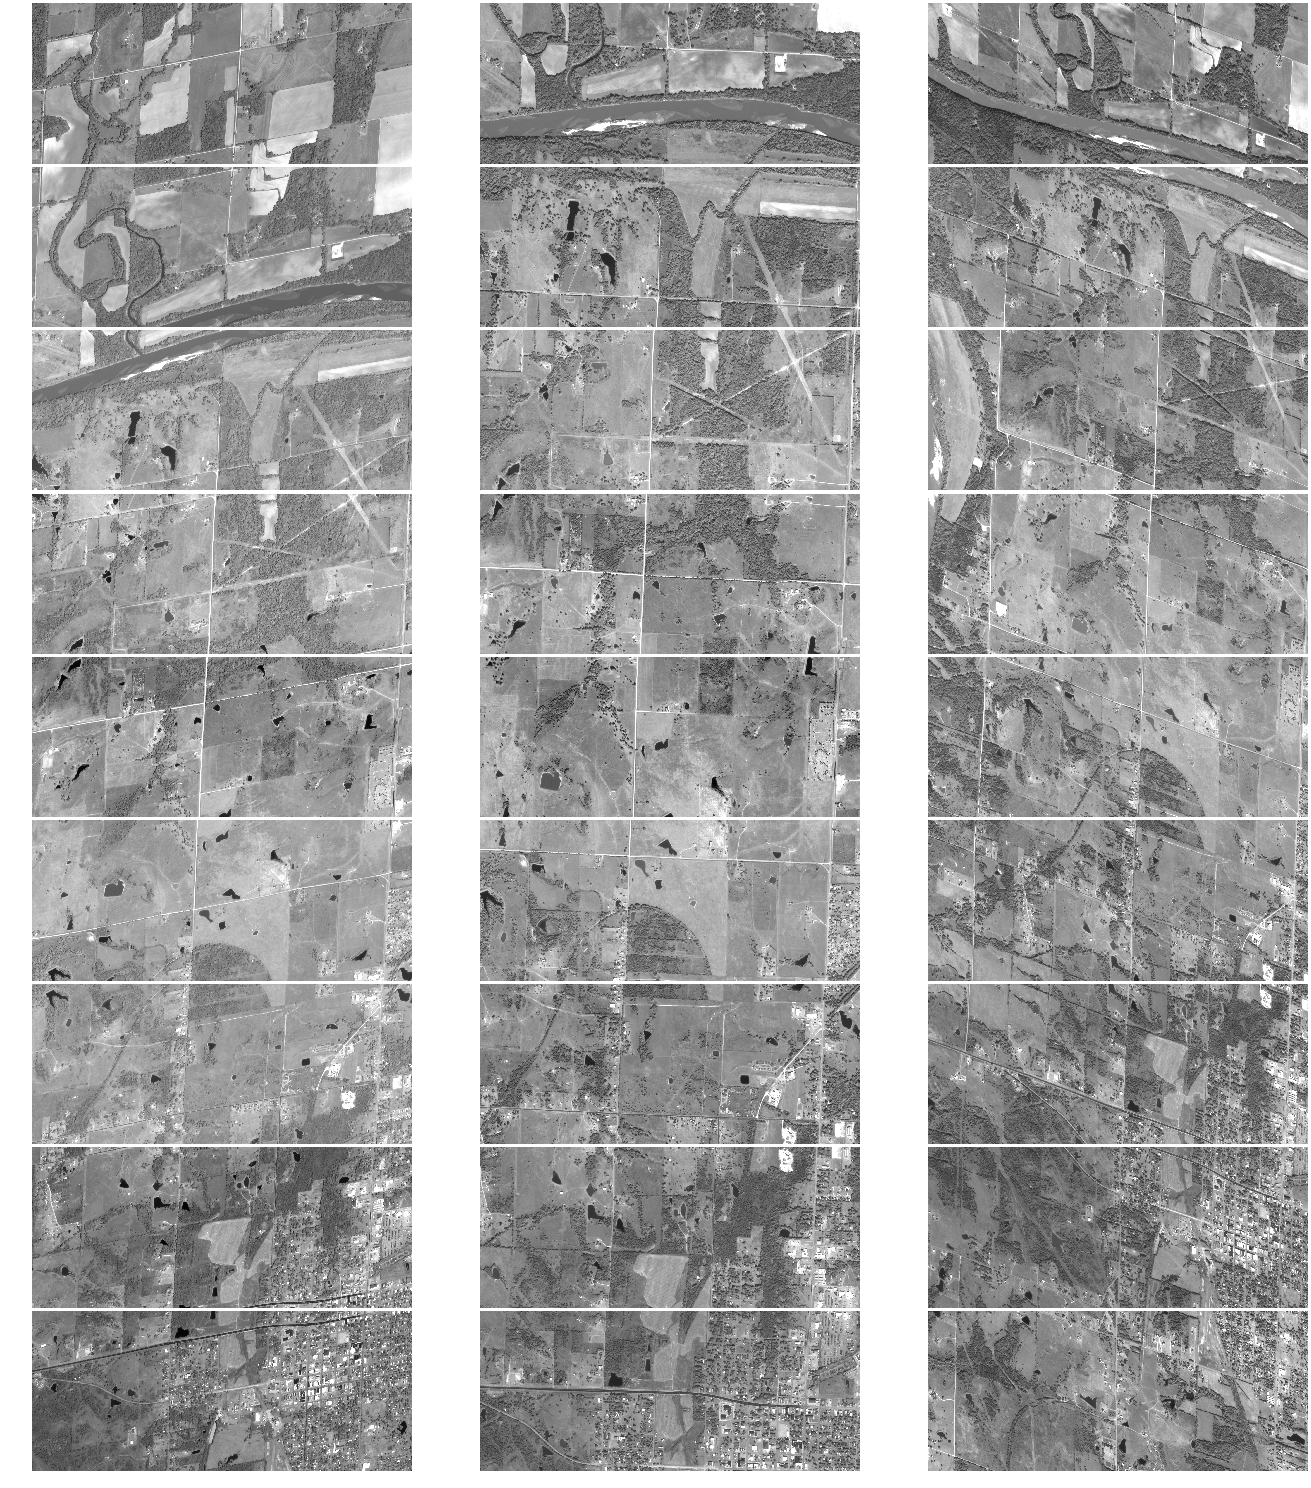
\includegraphics[width = 0.95\textwidth]{d3.png}
    \caption{Mosaic of d3. From left to right: 1Z, 8Z, 7Z}
    \label{fig_mosaic_d3}
\end{figure}


\appendix

\section{Rotations and translation}

In this part, we consider any point \((x, y) \in \mathbb{R}^2\). As translation and rotation do not commute, we will consider two cases: rotation followed by translation and translation followed by rotation, with \(R\) denoting the rotation of angle \(\theta\) and \(T\) denoting the translation of vector \((t_x, t_y)\). Naming \(f\) the resulting function.

\begin{align*}
    T &=
    \begin{pmatrix}
    1 & 0 & t_x \\
    0 & 1 & t_y \\
    0 & 0 & 1
    \end{pmatrix}
    \\
    R &=
    \begin{pmatrix}
    \cos \theta & -\sin \theta & 0 \\
    \sin \theta & \cos \theta & 0 \\
    0 & 0 & 1
    \end{pmatrix}
\end{align*}


\subsection{Rotation followed by a translation}
This happens when correcting the pointing error first with the rotation.

\begin{align*}
    f(\bm{x}) &= TR\bm{x} \\
    &=
    \begin{pmatrix}
    1 & 0 & t_x \\
    0 & 1 & t_y \\
    0 & 0 & 1
    \end{pmatrix}
    \cdot
    \begin{pmatrix}
    \cos \theta x - \sin \theta y \\
    \sin \theta x + \cos \theta y \\
    1
    \end{pmatrix}
    \\
    &=
    \begin{pmatrix}
    \cos \theta x - \sin \theta y + t_x\\
    \sin \theta x + \cos \theta y + t_y\\
    1
    \end{pmatrix}
\end{align*}

\subsection{Translation followed by a rotation}
This happens when correcting the pointing error first with the translation

\begin{align*}
    f(\bm{x}) &= RT\bm{x} \\
    &=
    \begin{pmatrix}
    \cos \theta & -\sin \theta & 0 \\
    \sin \theta & \cos \theta & 0 \\
    0 & 0 & 1
    \end{pmatrix}
    \cdot
    \begin{pmatrix}
    x + t_x \\
    y + t_y \\
    1
    \end{pmatrix} \\
    &=
    \begin{pmatrix}
    \cos \theta (x + t_x) - \sin \theta (y + t_y)\\
    \sin \theta (x + t_x) + \cos \theta (y + t_y)\\
    1
    \end{pmatrix}
\end{align*}


\bibliographystyle{plain}
\bibliography{biblio}
\end{document}

\end{document}
